% !TEX TS-program = XeLaTeX
% use the following command:
% all document files must be coded in UTF-8
\documentclass[spanish]{textolivre}
% build HTML with: make4ht -e build.lua -c textolivre.cfg -x -u article "fn-in,svg,pic-align"

\usepackage{graphicx} % no preâmbulo
\usepackage{longtable}
\usepackage{adjustbox}
\usepackage{array}
\usepackage{tabularx}
\journalname{Texto Livre}
\thevolume{18}
%\thenumber{1} % old template
\theyear{2025}
\receiveddate{\DTMdisplaydate{2024}{11}{13}{-1}} % YYYY MM DD
\accepteddate{\DTMdisplaydate{2025}{5}{5}{-1}}
\publisheddate{\DTMdisplaydate{2025}{8}{19}{-1}}
\corrauthor{Gustavo Herrera-Urízar}
\articledoi{10.1590/1983-3652.2025.55865}
%\articleid{NNNN} % if the article ID is not the last 5 numbers of its DOI, provide it using \articleid{} commmand 
% list of available sesscions in the journal: articles, dossier, reports, essays, reviews, interviews, editorial
\articlesessionname{reports}
\runningauthor{Herrera-Urízar, Moreno-González y Cisternas-Negrete} 
%\editorname{Leonardo Araújo} % old template
\sectioneditorname{Hugo Heredia Ponce}
\layouteditorname{Saula Cecília}

\title{Evaluación formativa con TIC en Filosofía: un estudio de caso en educación secundaria chilena}
\othertitle{Avaliação formativa com TIC em Filosofia: um estudo de caso no ensino médio chileno}
% if there is a third language title, add here:
\othertitle{Formative assessment with ICT in Philosophy: a case study in Chilean secondary education}

\author[1]{Gustavo Herrera-Urízar~\orcid{0000-0003-3546-8976}\thanks{Email: \href{mailto:gustavo.herrera@ub.edu}{gustavo.herrera@ub.edu}}}
\author[1]{Ainara Moreno-González~\orcid{0000-0002-8183-5434}\thanks{Email: \href{mailto:ainara.moreno@ub.edu}{ainara.moreno@ub.edu}}}
\author[2]{Souly Cisternas-Negrete~\orcid{0009-0006-4597-2569}\thanks{Email: \href{mailto:soulycist@gmail.com}{soulycist@gmail.com}}}
\affil[1]{Universidad de Barcelona, Barcelona, España.}
\affil[2]{Pontificia Universidad Católica de Valparaíso, Valparaíso, Chile.}

\addbibresource{article.bib}
% use biber instead of bibtex
% $ biber article

% used to create dummy text for the template file
\definecolor{dark-gray}{gray}{0.35} % color used to display dummy texts
\usepackage{lipsum}
\SetLipsumParListSurrounders{\colorlet{oldcolor}{.}\color{dark-gray}}{\color{oldcolor}}

% used here only to provide the XeLaTeX and BibTeX logos
\usepackage{hologo}

% if you use multirows in a table, include the multirow package
\usepackage{multirow}

% provides sidewaysfigure environment
\usepackage{rotating}

% CUSTOM EPIGRAPH - BEGIN 
%%% https://tex.stackexchange.com/questions/193178/specific-epigraph-style
\usepackage{epigraph}
\renewcommand\textflush{flushright}
\makeatletter
\newlength\epitextskip
\pretocmd{\@epitext}{\em}{}{}
\apptocmd{\@epitext}{\em}{}{}
\patchcmd{\epigraph}{\@epitext{#1}\\}{\@epitext{#1}\\[\epitextskip]}{}{}
\makeatother
\setlength\epigraphrule{0pt}
\setlength\epitextskip{0.5ex}
\setlength\epigraphwidth{.7\textwidth}
% CUSTOM EPIGRAPH - END

% to use IPA symbols in unicode add
%\usepackage{fontspec}
%\newfontfamily\ipafont{CMU Serif}
%\newcommand{\ipa}[1]{{\ipafont #1}}
% and in the text you may use the \ipa{...} command passing the symbols in unicode

% LANGUAGE - BEGIN
% ARABIC
% for languages that use special fonts, you must provide the typeface that will be used
% \setotherlanguage{arabic}
% \newfontfamily\arabicfont[Script=Arabic]{Amiri}
% \newfontfamily\arabicfontsf[Script=Arabic]{Amiri}
% \newfontfamily\arabicfonttt[Script=Arabic]{Amiri}
%
% in the article, to add arabic text use: \textlang{arabic}{ ... }
%
% RUSSIAN
% for russian text we also need to define fonts with support for Cyrillic script
% \usepackage{fontspec}
% \setotherlanguage{russian}
% \newfontfamily\cyrillicfont{Times New Roman}
% \newfontfamily\cyrillicfontsf{Times New Roman}[Script=Cyrillic]
% \newfontfamily\cyrillicfonttt{Times New Roman}[Script=Cyrillic]
%
% in the text use \begin{russian} ... \end{russian}
% LANGUAGE - END

% EMOJIS - BEGIN
% to use emoticons in your manuscript
% https://stackoverflow.com/questions/190145/how-to-insert-emoticons-in-latex/57076064
% using font Symbola, which has full support
% the font may be downloaded at:
% https://dn-works.com/ufas/
% add to preamble:
% \newfontfamily\Symbola{Symbola}
% in the text use:
% {\Symbola }
% EMOJIS - END

% LABEL REFERENCE TO DESCRIPTIVE LIST - BEGIN
% reference itens in a descriptive list using their labels instead of numbers
% insert the code below in the preambule:
%\makeatletter
%\let\orgdescriptionlabel\descriptionlabel
%\renewcommand*{\descriptionlabel}[1]{%
%  \let\orglabel\label
%  \let\label\@gobble
%  \phantomsection
%  \edef\@currentlabel{#1\unskip}%
%  \let\label\orglabel
%  \orgdescriptionlabel{#1}%
%}
%\makeatother
%
% in your document, use as illustraded here:
%\begin{description}
%  \item[first\label{itm1}] this is only an example;
%  % ...  add more items
%\end{description}
% LABEL REFERENCE TO DESCRIPTIVE LIST - END


% add line numbers for submission
%\usepackage{lineno}
%\linenumbers

\begin{document}
\maketitle

\begin{polyabstract}
\begin{abstract}
La enseñanza tradicional de la filosofía en la educación media y universitaria ha dependido principalmente de la evaluación sumativa, cuyo propósito constitutivo reside en la medición de los conocimientos disciplinares del estudiante y en la cuantificación de estos por medio una calificación que es directamente proporcional a los aciertos obtenidos. Esta investigación analiza las ventajas o desventajas que podría traer la implementación de la evaluación formativa con el acompañamiento de tecnologías de la información y comunicación (TIC) en la enseñanza de filosofía en Chile, evaluando su impacto en el rendimiento académico de los estudiantes y en las percepciones que expresó el profesorado respecto al desarrollo de la actividad. Esta investigación, de carácter cuantitativo y cualitativo, involucró a 80 estudiantes y tres profesores de filosofía de distintos centros educativos. En los últimos apartados de esta investigación, será posible ver cómo los resultados analizados estadísticamente evidencian un impacto positivo de la evaluación formativa con TIC en la atención y participación de los estudiantes, lo cual fue confirmado por el profesorado. De manera tal que no solo se permite, sino que se hace necesario resaltar el papel fundamental de las herramientas TIC y de las estrategias educativas que poseen un enfoque pedagógico lo suficientemente llamativo y contingente para promover un aprendizaje significativo que va más allá de la mera medición.

\keywords{Evaluación formativa\sep TIC\sep Enseñanza de la filosofía}
\end{abstract}

\begin{portuguese}
\begin{abstract}
O ensino tradicional da filosofia no ensino médio e universitário tem se baseado principalmente na avaliação sumativa, cujo objetivo constitutivo consiste em medir o conhecimento disciplinar do aluno e quantificá-lo através de uma nota diretamente proporcional às classificações obtidas. Esse estudo analisa as vantagens ou desvantagens que a implementação da avaliação formativa acompanhada pelas tecnologias da informação e da comunicação (TIC) poderia trazer ao ensino da filosofia no Chile, avaliando o seu impacto no desempenho acadêmico dos estudantes e nas percepções expressas pelos professores relativamente ao desenvolvimento da atividade. Esta investigação, de carácter quantitativo e qualitativo, envolveu 80 estudantes e três professores de filosofia de diferentes escolas. Nas últimas seções desta investigação, pode verificar-se que os resultados analisados estatisticamente mostram um impacto positivo da avaliação formativa com TIC na atenção e participação dos alunos, o que foi confirmado pelo pessoal docente. De tal forma que não só permite, mas também torna necessário destacar o papel fundamental das ferramentas TIC e das estratégias educativas que têm uma abordagem pedagógica suficientemente marcante e contingente para promover uma aprendizagem significativa que vai para além da medição.

\keywords{Avaliação formativa\sep TIC\sep Ensino de Filosofia}
\end{abstract}
\end{portuguese}
% if there is another abstract, insert it here using the same scheme

\begin{english}
\begin{abstract}
The conventional pedagogy of philosophy in secondary and university education has relied mainly on summative assessment, whose fundamental purpose lies in the measurement of the student’s disciplinary knowledge and its quantification by means of a grade that is directly proportional to the successes obtained. This study analyzes the advantages or disadvantages that the implementation of formative assessment with the accompaniment of information and communication technologies (ICT) could bring to the teaching of philosophy in Chile, evaluating its impact on the academic performance of students and the perceptions expressed by teachers regarding the development of the activity. This research, of a quantitative and qualitative nature, involved 80 students and three philosophy teachers from different educational centers. In the last sections of this research, it can be seen that the statistically analyzed results show a positive impact of the formative evaluation with ICT on the students’ attention and participation, which was confirmed by the teachers. In such a way, it is not only allowed, but also necessary to highlight the fundamental role of ICT tools and educational strategies that have a pedagogical approach sufficiently striking and contingent to promote meaningful learning that goes beyond measurement.

\keywords{Formative assessment\sep ICT\sep Philosophy teaching}
\end{abstract}
\end{english}
% if there is another abstract, insert it here using the same scheme
\end{polyabstract}

\section{Introducción}
La evaluación formativa ha adquirido una importancia significativa en los últimos años como una estrategia educativa que trasciende una medición simplista del rendimiento académico, promoviendo un proceso de retroalimentación constante que impulsa la autorregulación y mejora el aprendizaje de los estudiantes \cite{gallardo-fuentes2020}. Incluso, si bien en Chile se promulgó un Decreto educativo, llamado Decreto 67 \cite{bcn2018decreto67}, para forzar su entrada en los colegios, no fue hasta el término de la pandemia que el nombre de evaluación formativa comenzó a resonar más fuertemente en las aulas de clases. Obligando a las escuelas a fomentar cursos de capacitación docente y a incorporar en sus planificaciones instancias que permitiesen reforzar el aprendizaje y autonomía de sus estudiantes para apoyarlos en sus procesos particulares sin la necesidad de calificarlos. En la educación secundaria, este enfoque resulta esencial, ya que permite a los estudiantes identificar sus fortalezas y áreas de mejora de forma contínua, a lo largo de su trayectoria educativa. Además, estudios recientes indican que la evaluación formativa incrementa el compromiso de los estudiantes al involucrarlos activamente en su proceso de aprendizaje, desarrollando habilidades críticas que van más allá de la memorización de contenidos y favoreciendo un aprendizaje más profundo y reflexivo \cite{bizarro2019}.

La implementación de la evaluación formativa en las aulas no solo transforma la concepción de la evaluación, sino que también modifica la dinámica entre docentes y estudiantes, fomentando una relación basada en la colaboración y la mejora continua \cite{hidalgo2021}. En este sentido, \textcite{copado2022} argumenta que la evaluación formativa permite a los docentes ajustar sus estrategias pedagógicas en tiempo real, adaptándolas a las necesidades y al ritmo de aprendizaje de cada estudiante. Este enfoque es especialmente relevante en la educación secundaria, donde los estudiantes se encuentran en una fase crucial de construcción de su identidad académica y necesitan un entorno que les permita explorar sus competencias sin la presión de una calificación final. Así, la evaluación formativa se convierte en un espacio seguro que facilita el desarrollo de habilidades de autorreflexión y autorregulación, componentes esenciales para el éxito académico en etapas avanzadas.

Además, la evaluación formativa ha demostrado ser una herramienta poderosa para el desarrollo de habilidades metacognitivas, alentando a los estudiantes a reflexionar sobre su proceso de aprendizaje y a definir sus propias metas académicas \cite{galarza-salazar2021}. En un estudio sobre prácticas pedagógicas, \textcite{mendoza2020} destacan que la evaluación formativa en la educación secundaria promueve una cultura de aprendizaje continuo en la que los estudiantes no buscan únicamente aprobar, sino comprender profundamente los contenidos. De esta forma, la evaluación formativa se destaca como estrategia esencial para fomentar el aprendizaje autónomo en los estudiantes, adquiriendo especial relevancia en la enseñanza de la filosofía, donde se espera que los estudiantes desarrollen competencias críticas y reflexivas.

La evaluación formativa, sin embargo, enfrenta grandes desafíos en la educación secundaria y universitaria, puesto que históricamente las instituciones han implementado principalmente evaluaciones de carácter sumativo \cite{hidalgo2021}. En el ámbito de la educación primaria y en la formación inicial del profesorado, se ha revisado sistemáticamente la relación entre la evaluación formativa y la adquisición de competencias docentes, encontrando beneficios significativos en el desarrollo de habilidades en los estudiantes de educación física \cite{jihuallanca2023}. En el contexto chileno, también se ha investigado cómo los docentes universitarios en programas de formación de profesores entienden y practican la evaluación formativa \cite{orellana2020}. Por tanto, la evaluación formativa apoyada del uso de TIC se inserta dentro de un amplio contexto de estudios que exploran esta práctica en diferentes niveles educativos y hacen uso de diversas didácticas adecuadas para asegurarse de guiar el aprendizaje particular de cada alumno sin dejar de lado a nadie. Preocupándose no solo del logro académico, sino también de enseñar a valorar el proceso de aprendizaje por el cual transita toda la basta diversidad de estudiantes. 

En la enseñanza de la filosofía en la educación secundaria, la evaluación formativa se presenta como un enfoque particularmente adecuado, ya que la naturaleza abstracta e interdisciplinaria de la asignatura requiere habilidades de análisis crítico y reflexión que suelen quedar fuera del alcance de las evaluaciones sumativas tradicionales \cite{orellana2020}. A diferencia de otras materias, donde es posible medir los conocimientos específicos a través de pruebas estandarizadas, la filosofía demanda un enfoque evaluativo que fomente la capacidad de cuestionar, argumentar y construir conocimiento propio. En este contexto, \textcite{mendoza2020} enfatizan que la evaluación formativa permite que los estudiantes avancen en su comprensión mediante retroalimentación constante, promoviendo un diálogo continuo entre docentes y estudiantes, dado a que proporciona un ambiente distendido en el cual equivocarse supone un paso más dentro del aprendizaje.

La evaluación formativa en filosofía, entonces, no solo mejora el rendimiento académico; también busca transformar la experiencia educativa en un proceso significativo. \textcite{lopez-pastor2011} sostiene que la evaluación formativa ofrece un entorno de aprendizaje en el que los estudiantes pueden explorar temas complejos sin temor a ser juzgados exclusivamente por aciertos o errores, sino por su capacidad de razonamiento y análisis. Este enfoque permite que los estudiantes no solo asimilen conceptos filosóficos, sino que también aprendan a cuestionarlos, generando un proceso reflexivo que fortalece sus habilidades de pensamiento crítico. Además, en un contexto educativo en el que la filosofía ha sido evaluada predominantemente mediante enfoques sumativos, la integración de estrategias híbridas que combinen tanto la evaluación formativa como la sumativa, especialmente a través del uso de TIC, posibilita un enfoque más integral y dinámico \cite{black2009, nicol2006}. Esta combinación no solo amplía las oportunidades de interacción y compromiso del estudiantado, sino que también facilita la recolección y sistematización de datos que permiten una retroalimentación continua, asegurando una mayor coherencia entre los diferentes instrumentos evaluativos \cite{sadler1989}.

De hecho, \textcite{gallardo-fuentes2017} subrayan que las TIC pueden facilitar el proceso de evaluación formativa en filosofía al crear espacios de retroalimentación inmediata y personalizada, que se adaptan al ritmo de cada estudiante. La elección de la filosofía como objeto de estudio en esta investigación responde a la necesidad de adaptar las prácticas evaluativas a las exigencias de la disciplina, explorando cómo la evaluación formativa con TIC puede enriquecer el proceso de enseñanza-aprendizaje en la educación secundaria chilena.

La implementación de la evaluación formativa en el ámbito educativo es fundamental para promover un cambio de paradigma, pasando de una cultura centrada en exámenes a una cultura de evaluación que fomente el aprendizaje continuo y la autorregulación en los estudiantes \cite{bizarro2019}. Esta transición es crucial para romper con el enfoque tradicional que limita la creatividad y la innovación de los estudiantes al enfocarse en la reproducción de conocimientos \cite{mendoza2020}. En el marco de las competencias, la evaluación formativa busca superar las limitaciones de las prácticas evaluativas convencionales en el aula, permitiendo que la evaluación se oriente hacia el aprendizaje y contribuya a mejorar el proceso de enseñanza \cite{galarza-salazar2021}.

La evaluación formativa, en este sentido, facilita la creación de espacios de confianza entre el alumno y el docente, donde el estudiante se siente seguro para expresar sus dudas, explorar sus errores y recibir retroalimentación constructiva. Este ambiente propicia un aprendizaje en el que el estudiante no solo busca ``aprobar", sino adquirir y consolidar conocimientos que le permitan avanzar de forma autónoma. En el contexto de la enseñanza de la filosofía, donde el pensamiento crítico y la reflexión son esenciales, estos espacios de evaluación formativa son particularmente valiosos, ya que permiten a los estudiantes desarrollar habilidades de análisis y cuestionamiento, habilidades que los preparan para el pensamiento filosófico y el aprendizaje continuo \cite{galarza-salazar2021}.

Frente a estos desafíos, la implementación de la evaluación formativa con TIC se convierte en una herramienta innovadora que puede revolucionar la enseñanza de la filosofía. En una investigación reciente sobre la evaluación formativa y el uso de TIC en el currículo de filosofía en educación secundaria en Chile, se identificó como una problemática fundamental la escasa participación de los estudiantes, atribuible en gran medida a una cultura académica que valora principalmente la calificación \cite{lombardo-bertolini2024}. Esta lógica desprendida de la costumbre al refuerzo positivo que implica en ciertas ocasiones la evaluación sumativa ha derivado en una baja motivación para participar activamente en procesos de retroalimentación, ya que los estudiantes perciben que estos espacios no tienen un impacto directo en sus calificaciones. La implementación de TIC como parte de la evaluación formativa busca transformar este escenario, captando la atención del alumnado a través de plataformas digitales que, además de organizar el aprendizaje, ofrecen una experiencia interactiva que fomenta la participación y el compromiso.

Esta investigación explora la incorporación de plataformas virtuales y herramientas digitales orientadas a transformar el enfoque tradicional punitivo de la evaluación, integrando el proceso metacognitivo del estudiante como un eje central de su formación. El objetivo es fomentar el desarrollo de habilidades de autorregulación y motivación, promoviendo un aprendizaje significativo y autónomo. A través de estas herramientas, los docentes pueden presentar actividades evaluativas que no solo miden el conocimiento, sino que también motivan a los estudiantes a participar en la coevaluación y autoevaluación de sus habilidades \cite{mendoza2020}. En este marco, las TIC no solo facilitan el acceso a actividades interactivas, sino que permiten un proceso de aprendizaje dinámico, en el que la retroalimentación y el acompañamiento pedagógico se convierten en pilares fundamentales para el desarrollo académico y personal del estudiante \cite{lopez-pastor2011}.

Finalmente, en un contexto en el que la filosofía y otras asignaturas similares suelen estar ancladas a modelos tradicionales de evaluación, el uso de una evaluación formativa con apoyo de TIC representa un cambio de paradigma que responde a las necesidades educativas contemporáneas. A través de esta investigación se busca demostrar cómo, mediante la evaluación formativa apoyada en tecnología, es posible enriquecer no solo el aprendizaje en filosofía, sino también transformar las prácticas pedagógicas y el papel de los estudiantes en su propio proceso de aprendizaje.

En este contexto surgen naturalmente algunas preguntas clave: ¿Constituyen la evaluación formativa y el uso de TIC herramientas decisivas para motivar la participación en el aula? ¿Hasta qué punto son útiles las TIC para evaluar los conocimientos filosóficos de cada estudiante? Así, el objetivo de esta investigación es analizar la implementación de la evaluación formativa apoyada por tecnologías digitales de la información y la comunicación, considerando tanto los resultados obtenidos por los estudiantes como las percepciones del profesorado en el contexto de la educación secundaria en Chile.


\section{Metodología}
La investigación propuesta adopta un enfoque mixto, combinando métodos cuantitativos y cualitativos para evaluar exhaustivamente el impacto de las evaluaciones formativas en la enseñanza media. En primer lugar, desde una perspectiva cuantitativa, se llevó a cabo un análisis detallado de los resultados de las evaluaciones formativas mediante el uso de Nearpod, una plataforma digital que permitió la aplicación periódica de actividades evaluativas cada dos semanas durante un semestre académico. Estas evaluaciones incluyeron cuestionarios interactivos, actividades de arrastrar y soltar y ejercicios de reflexión crítica, diseñados para monitorear el progreso del estudiantado en tiempo real. Los resultados obtenidos a través de Nearpod se procesaron mediante técnicas estadísticas avanzadas, lo que permitió identificar tendencias significativas y áreas de mejora específicas en el desempeño estudiantil \cite{yazidi2023}.

Por otro lado, desde una perspectiva cualitativa, se realizó una exploración de las percepciones y experiencias de los profesores de enseñanza media respecto a la implementación de evaluaciones formativas digitales. A través de entrevistas semiestructuradas y grupos focales, se profundizó en las estrategias de retroalimentación utilizadas. Los procedimientos de \textit{feedback} se llevaron a cabo al finalizar cada sesión evaluativa en Nearpod, incluyendo reuniones de retroalimentación individuales y grupales, donde se analizó el desempeño de los estudiantes y se ofrecieron recomendaciones personalizadas para abordar las áreas de dificultad identificadas. La metodología cualitativa empleada se basó en un enfoque de análisis de contenido siguiendo las pautas establecidas por \textcite{sandvoll2014}, lo que permitió identificar temas emergentes en las prácticas de retroalimentación y adaptación de las actividades evaluativas al contexto específico de cada grupo de estudiantes.

Además, la investigación se ajustó rigurosamente a las normas éticas y de protección de datos, obteniendo la aprobación del comité de ética de la Vicerrectoría Académica, específicamente de la Unidad de Mejoramiento de la Docencia Universitaria, bajo el código del proyecto 2023.01.INV.FIL.01. Esta aprobación aseguró el cumplimiento de los principios éticos en la gestión de datos y en la interacción con los participantes, garantizando el consentimiento informado, la confidencialidad y el anonimato. Se enfatizó, además, en la adaptación contextual de las actividades formativas a partir de las necesidades detectadas en cada grupo de estudiantes, lo que contribuyó al ajuste continuo de las estrategias evaluativas a lo largo de la investigación.

Finalmente, es importante destacar que la colaboración interdisciplinaria entre docentes de enseñanza media y profesores universitarios especializados en formación docente en filosofía no solo enriqueció el diseño de las evaluaciones, sino que también promovió un intercambio de conocimientos y experiencias clave. Este enfoque integrador fomentó la innovación pedagógica y la mejora continua en el ámbito educativo, consolidando un modelo híbrido de evaluación formativa que articula la evaluación continua y la sumativa para potenciar el aprendizaje de los estudiantes.

\subsection{Percepción inicial sobre los contenidos fundamentales de filosofía}

Se realizaron dos grupos focales, uno de ellos involucró la participación de dos profesores y una profesora de educación secundaria, mientras que en el otro se constituyó con dos profesores de formación inicial docente en filosofía para conocer su percepción sobre los contenidos fundamentales del currículo de la asignatura en cuestión. Durante el desarrollo de los grupos focales, se identificaron temas o conceptos que se consideran como ``más importantes", junto con las respectivas dificultades que encuentran al tratar de enseñarlos o incluso aprenderlos \cite{lombardo-bertolini2024} (\Cref{tab-1}).

%--- CÓDIGO DA TABELA 1 ---%
\begin{table}[h!]
\centering
\caption{Muestra de participantes.}\label{tab-1}
\begin{tabularx}{\textwidth}{lXlXl}
\toprule
Identificador & Perfil & Sexo & Vinculación Institucional & Modalidad \\
\midrule
PROF1 & Académico Historia de la Filosofía Antigua & Hombre & Universidad & Virtual \\
PROF2 & Académico Historia de la Filosofía Medieval & Hombre & Universidad & Virtual \\
PROF3 & Profesor & Hombre & Colegio & Virtual \\
PROF4 & Profesora & Mujer & Colegio & Virtual \\
PROF5 & Profesor & Hombre & Colegio & Virtual \\
\bottomrule
\end{tabularx}
\source{Elaboración propia.}
\end{table}

\subsection{Análisis de las planificaciones y programas de filosofía}
Se analizaron las planificaciones y programas de filosofía de los profesores de enseñanza media y de los profesores de enseñanza universitaria para identificar los objetivos de aprendizaje, resultados de aprendizaje, las metodologías de enseñanza y los instrumentos de evaluación utilizados para comparar los diferentes enfoques y detectar las posibles áreas de articulación, convergencia o divergencia (\Cref{tab-2}).

%--- CÓDIGO DA TABELA 2 ---%
\begin{table}[h!]
\centering
\caption{Muestra de documentos.}\label{tab-2}
\small
\begin{tabularx}{\textwidth}{lXlX}
\toprule
Identificador & Nombre de documento & Tipo de documento & Nivel de educación \\
\midrule
Texto 1 & Objetivos de aprendizaje: Habilidades transversales 3° y 4° Medio -- Bases Curriculares 3° y 4° Medio & Currículum nacional de Chile & 3° y 4° Medio \\
Texto 2 & Objetivos de aprendizaje: Conocimiento y comprensión 3º Medio -- Bases Curriculares 3° y 4° Medio & Currículum nacional de Chile & 3° Medio \\
Texto 3 & Objetivos de aprendizaje: Conocimiento y comprensión 4º Medio -- Bases Curriculares 3° y 4° Medio & Currículum nacional de Chile & 4° Medio \\
Texto 4 & Planificación de Asignatura: Seminario de Filosofía & Planificación de Centro 1 & 3° y 4° Medio \\
Texto 5 & Planificación de Asignatura: Filosofía común & Planificación de Centro 2 & 3° Medio \\
Texto 6 & Planificación de Asignatura: Filosofía común & Planificación de Centro 3 & 4° Medio \\
Texto 7 & Planificación de Asignatura: Filosofía común & Planificación de Centro 1 & 4° Medio \\
Texto 8 & Historia de la filosofía antigua 1 & Programa de asignatura & 1º año de FID en pedagogía en filosofía \\
Texto 9 & Historia de la filosofía antigua 2 & Programa de asignatura & 1º año de FID en pedagogía en filosofía \\
Texto 10 & Historia de la filosofía medieval 1 & Programa de asignatura & 2º año de FID en pedagogía en filosofía \\
Texto 11 & Historia de la filosofía medieval 2 & Programa de asignatura & 2º año de FID en pedagogía en filosofía \\
\bottomrule
\end{tabularx}
\source{Elaboración propia.}
\end{table}

\subsection{Borrador en conjunto de instrumento de evaluación formativa}
En base a la información obtenida en los pasos 1 y 2, se elaboró un borrador en conjunto del instrumento de evaluación formativa. El instrumento incluyó una variedad de preguntas y actividades que permiten evaluar los diferentes aspectos del aprendizaje de la filosofía, tales como el conocimiento conceptual, la comprensión crítica, las habilidades de argumentación y la capacidad de análisis. 

Dado que el enfoque de esta investigación es de naturaleza pedagógica, el instrumento desarrollado para la evaluación formativa con TIC se diseñó principalmente como una herramienta educativa, orientada a mejorar la enseñanza y aprendizaje de la filosofía en el contexto de la educación secundaria. Este instrumento no pretende ser una herramienta de investigación rigurosa, sino una experiencia pedagógica creada para promover el compromiso y la participación de los estudiantes en el proceso de aprendizaje. No obstante, para asegurar su efectividad en el aula, se realizó un proceso de revisión y ajuste que permitió afinar los elementos del instrumento y adaptarlos al contexto específico de los estudiantes de secundaria.

En esta línea, el instrumento fue revisado por un grupo de docentes secundarios y universitarios, quienes evaluaron la claridad de los ítems y su pertinencia en relación con los objetivos de aprendizaje planteados para la asignatura de filosofía. Este proceso permitió realizar ajustes en la formulación de preguntas y actividades para asegurar que fueran comprensibles y motivadoras para los estudiantes, promoviendo su interacción activa con los contenidos filosóficos \cite{gutiérrez2019}. La herramienta fue diseñada para funcionar en la plataforma Nearpod, lo cual permitió integrar actividades interactivas que facilitan la retroalimentación en tiempo real y generarán un ambiente de aprendizaje dinámico y atractivo.

Además, se realizó una prueba piloto con un grupo pequeño de estudiantes para observar su reacción y nivel de participación en las actividades propuestas. Este piloto reveló áreas de mejora en la presentación de algunos contenidos y en la claridad de las instrucciones, lo que llevó a realizar ajustes adicionales que optimizaron la experiencia pedagógica. Así, el proceso de revisión y ajuste del instrumento contribuyó a garantizar que su aplicación en el aula cumpliera con los objetivos de fomentar la reflexión crítica y el diálogo filosófico, promoviendo un aprendizaje significativo en un entorno digital \cite{flores2021}.

\subsection{Digitalización del instrumento evaluativo}
Se confeccionó, con ayuda de los dos profesores universitarios de filosofía, una herramienta evaluativa en la plataforma virtual de Nearpod, la cual fue seleccionada con el fin de crear exposiciones interactivas y llamativas para los alumnos. En este elemento digital ellos pueden responder preguntas abiertas o de selección múltiple, según sea la actividad que haya sido incorporada; así como interactuar con herramientas que se hayan dispuesto dentro de la presentación digitalizada, ya sean vídeos, links, fotografías estáticas y con movimiento, pizarras digitales para rayar sobre las diapositivas, u otras. Dentro de dicha evaluación se incorporaron preguntas abiertas, en las que los alumnos tuvieron plena libertad para responder y preguntas cerradas que les obligó a escoger sólo una de las opciones asignadas por cada ítem. Si bien la idea inicial de esta actividad era examinar los saberes y conocimientos que los alumnos tenían acerca de los contenidos filosóficos antiguos y medievales para entregarles una retroalimentación individual y grupal respecto a su desempeño, el objetivo central detrás de la evaluación era observar la reacción que tenían los estudiantes al momento de participar: medir su participación y cuantificar su interés por la plataforma. Por estas razones, fue necesaria la guía y conducción de cada profesor involucrado, de manera tal que el instrumento pudiera ser adaptado sin mayores impedimentos a los distintos contextos escolares (\Cref{fig-1,fig-2,fig-3}). 

%--- CÓDIGO DA FIGURA 1 ---%
\begin{figure}[h!]
    \centering
    \begin{minipage}{0.77\linewidth}
    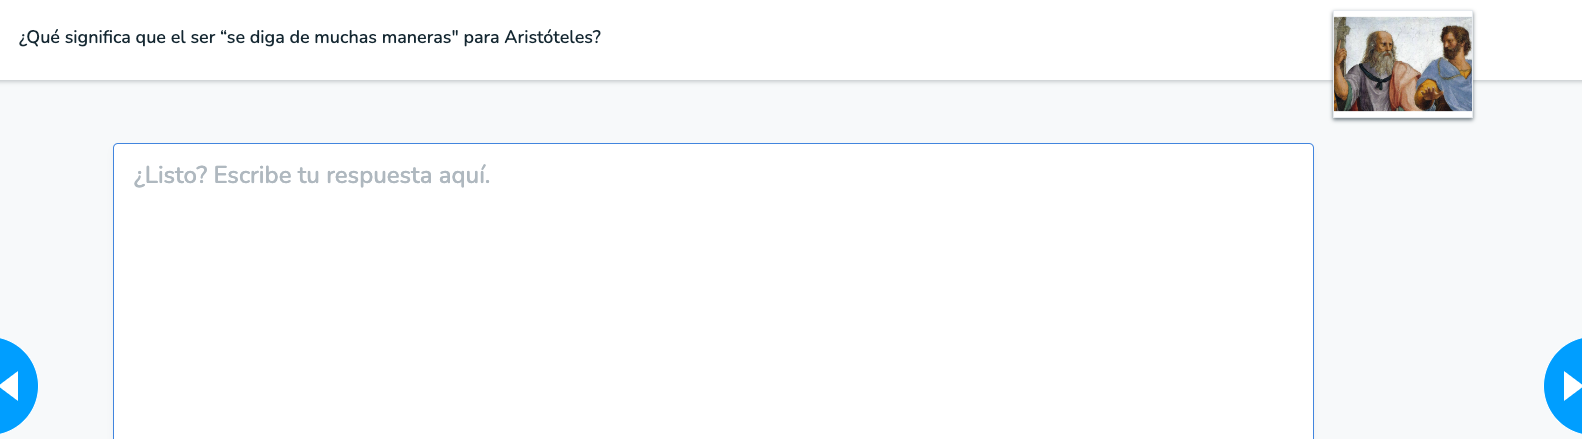
\includegraphics[width=\linewidth]{imagens/image1.png}
    \caption{Captura de evaluación formativa N.º1.}
    \label{fig-1}
    \source{Elaboración propia desde \url{https://app.nearpod.com/}.}
    \end{minipage}
\end{figure}

%--- CÓDIGO DA FIGURA 2 ---%
\begin{figure}[h!]
    \centering
    \begin{minipage}{0.77\linewidth}
    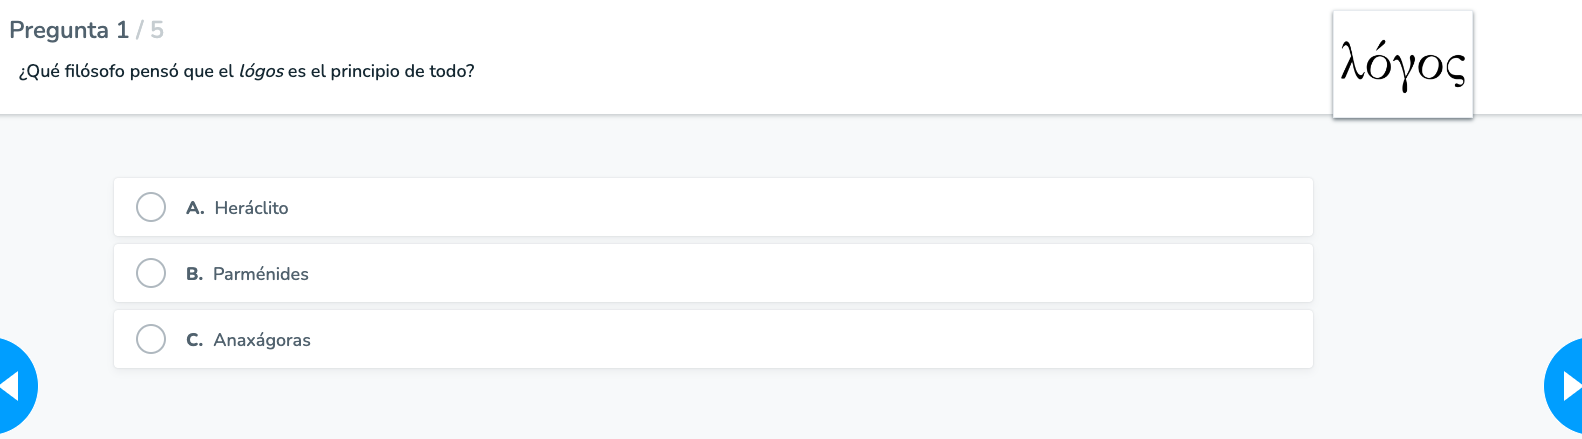
\includegraphics[width=\linewidth]{imagens/image3.png}
    \caption{Captura de evaluación formativa N.º1.}
    \label{fig-2}
    \source{Elaboración propia desde \url{https://app.nearpod.com/}.}
    \end{minipage}
\end{figure}

%--- CÓDIGO DA FIGURA 3 ---%
\begin{figure}[h!]
    \centering
    \begin{minipage}{0.77\linewidth}
    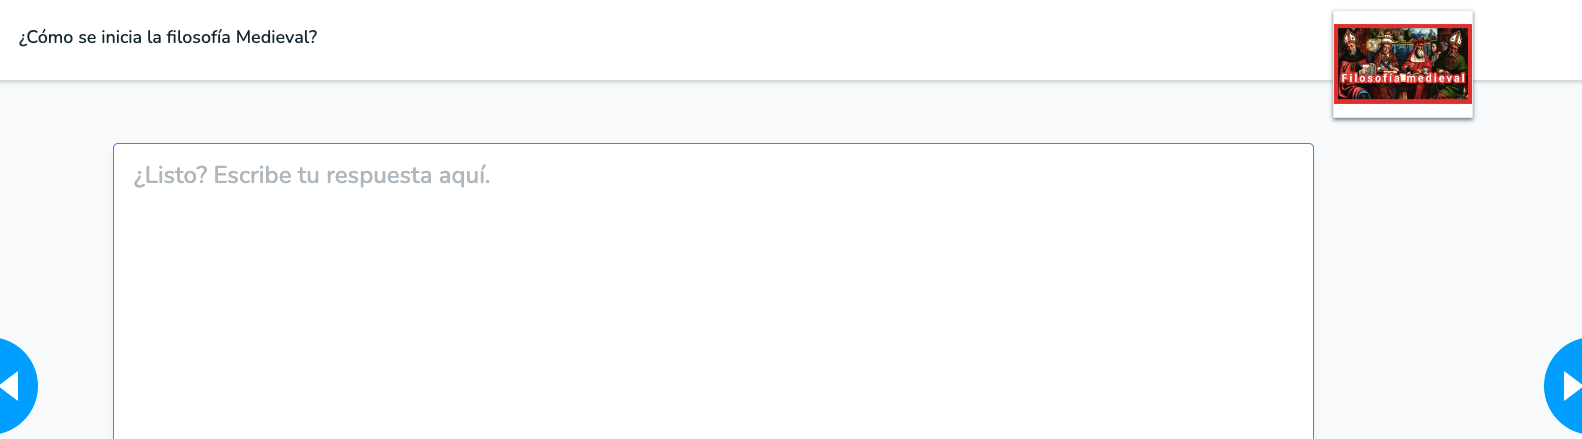
\includegraphics[width=\linewidth]{imagens/image2.png}
    \caption{Captura de evaluación formativa N.º1.}
    \label{fig-3}
    \source{Elaboración propia desde \url{https://app.nearpod.com/}.}
    \end{minipage}
\end{figure}

\subsection{Aplicación del instrumento en colegios}
Se seleccionaron tres colegios de educación media o secundaria, de acuerdo con el interés presentado en la iniciativa luego de realizar una convocatoria dirigida a todos los centros de la región de Valparaíso (Chile), para aplicar el instrumento de evaluación formativa. Y, entre las tres escuelas que se involucraron en el proyecto, se logró obtener la participación de 80 alumnos en total (\Cref{tab-3}).

%--- CÓDIGO DA TABELA 3 ---%
\begin{table}[h!]
\centering
\begin{threeparttable}
\caption{Características del estudiantado.}\label{tab-3}
\begin{tabular}{lcl}
\toprule
Identificador & Número de estudiantes & Género de estudiante \\
\midrule
Colegio 1 & 25 & 25 hombres \\
Colegio 2 & 23 & 14 mujeres -- 9 hombres \\
Colegio 3 & 32 & 21 mujeres -- 11 hombres \\
\bottomrule
\end{tabular}
\source{Elaboración propia.}
\end{threeparttable}
\end{table}

\subsection{Evaluación de los resultados}
Se analizaron los datos obtenidos de la aplicación del instrumento de evaluación formativa. Identificando los patrones y tendencias en los resultados, así como las fortalezas y debilidades de los estudiantes en el aprendizaje de los contenidos filosóficos; comparando los resultados de los diferentes colegios y grupos de estudiantes para discriminar el compromiso o impacto que pudiera tener cada contexto con el aprendizaje individual de cada participante.

\subsection{Percepción del profesorado de enseñanza media sobre la implementación de evaluación formativa con uso de TIC}
Se realizaron entrevistas a los profesores de enseñanza media que participaron en la investigación para conocer su percepción sobre la implementación de la evaluación formativa con uso de TIC, identificando aspectos positivos, negativos y recomendaciones generales para mejorar el procedimiento de la experiencia en el futuro. 

La construcción de este proceso se basa en la estrecha colaboración entre profesores de educación media y de formación inicial docente en filosofía. Juntos, diseñaron un proceso sistemático y participativo para crear una evaluación formativa que fomente la autocrítica y el análisis en los estudiantes. Aprovechando las ventajas que ofrecen las TIC, como la entretención y la armonía visual, facilitan la implementación eficiente de instancias formativas. Este tipo de evaluación permite identificar rápidamente las fortalezas y debilidades de los estudiantes en la asignatura de filosofía, favoreciendo tanto la organización de la información como una respuesta visible en la participación activa y, por lo tanto, una retroalimentación efectiva (\Cref{fig-4}).

%--- CÓDIGO DA FIGURA 4 ---%
\begin{figure}[h!]
    \centering
    \begin{minipage}{0.8\linewidth}
    
\includegraphics[width=\linewidth]{imagens/image4.png}
    \caption{Proceso metodológico.}\label{fig-4}
    \source{Elaboración propia.}
    \end{minipage}
\end{figure}

A partir de la evidencia obtenida hemos abordado tres dimensiones de análisis asociadas a los resultados: 1. Resultados de la evaluación formativa con uso de TIC; 2. Percepciones del profesorado sobre el proceso de implementación del instrumento; 3. Percepciones del profesorado sobre los resultados de la evaluación formativa con uso de TIC.

\section{Resultados}

\subsection{Resultados de la evaluación formativa con uso de TIC}
A continuación, se analizan los datos de participación y respuestas correctas en la evaluación formativa aplicada a los estudiantes de tres colegios. Se compara el rendimiento académico entre los diferentes centros educativos y se obtienen afirmaciones que puedan ser útiles para la mejora de la calidad educativa (\Cref{tab-4}).

%--- CÓDIGO DA TABELA 4 ---%
\begin{table}[h!]
\centering
\begin{threeparttable}
\caption{Participación y respuestas correctas del cuestionario.}\label{tab-4}
\begin{tabular}{lcc}
\toprule
Identificador & \% Participación & \% Correcto del cuestionario \\
\midrule
Colegio 1 & 75\% & 61\% \\
Colegio 2 & 67\% & 60\% \\
Colegio 3 & 65\% & 58\% \\
\bottomrule
\end{tabular}
\source{Elaboración propia.}
\end{threeparttable}
\end{table}

La tabla proporcionada muestra el porcentaje de participación y el porcentaje de respuestas correctas en el cuestionario para cada uno de los tres colegios. Se observa que la participación es alta en todos los colegios, con un promedio del 69\%. Sin embargo, existe una ligera variación entre los centros, siendo el Colegio 1 el que presenta la mayor participación (75\%) y el Colegio 3 el que tiene la menor (65\%).

En cuanto al porcentaje de respuestas correctas, el promedio general es del 59\%. De nuevo, se observan diferencias entre los colegios, con el Colegio 1 obteniendo el mejor resultado (61\%) y el Colegio 3 el más bajo (58\%).

Los datos de la investigación sugieren que, en general, existe una buena participación de los estudiantes en el cuestionario. Sin embargo, se observan algunas diferencias entre los colegios, tanto en términos de participación como de rendimiento académico. El Colegio 1 se destaca por tener la mayor participación y el mejor porcentaje de respuestas correctas, mientras que el Colegio 3 presenta los resultados más bajos en ambas categorías.

Para evaluar la efectividad de la evaluación formativa digital de Nearpod que se incorporó en la asignatura de filosofía de los tres colegios participantes, primero se consideraron los porcentajes de participación que se obtuvo en la actividad de filosofía antigua y en la actividad de filosofía medieval. Cabe destacar que la calidad del compromiso de los estudiantes se catalogó en: (1) excelentemente logrado, (2) bien logrado, (3) vagamente logrado y (4) no participó. Además, el porcentaje se calculó en base a la cantidad de alumnos que se inscribieron en la plataforma, los cuales fueron específicamente 40 en ambas materias (filosofía antigua y filosofía medieval) (\Cref{tab-5}).

%--- CÓDIGO DA TABELA 5 ---%
\begin{table}[h!]
\centering
\begin{threeparttable}
\caption{Participación de los y las estudiantes en las evaluaciones formativas.}\label{tab-5}
\begin{tabular}{lcc}
\toprule
Grado de participación & Filosofía Antigua & Filosofía Medieval \\
\midrule
Excelentemente logrado & 37{,}5\% & 52{,}5\% \\
Bien logrado & 10\% & 7{,}5\% \\
Vagamente logrado & 42{,}5\% & 30\% \\
No participó & 10\% & 10\% \\
Total & 100\% & 100\% \\
\bottomrule
\end{tabular}
\source{Elaboración propia.}
\end{threeparttable}
\end{table}

Al comparar los resultados, observamos que, si bien una parte significativa de los estudiantes participó activamente en la evaluación y respondió a todas las preguntas, en el caso de la filosofía antigua, un 42,5\% no se tomó la actividad del todo responsablemente, lo que representa casi la mitad del curso. Un fenómeno similar ocurrió en filosofía medieval, pero el porcentaje de participaciones incompletas no superó el 30\%, lo que indica una mayor afinidad de los estudiantes por esta disciplina.

Para contextualizar los resultados, se presentan los datos desglosados por centros educativos y por sexo, permitiendo observar de manera más detallada el nivel de participación y el porcentaje de respuestas correctas alcanzado por los y las estudiantes. A su vez, se examinan los resultados vinculándolos con los objetivos, contenidos, criterios de evaluación y resultados de aprendizaje establecidos para cada actividad formativa. Esta estructura analítica permite no solo evaluar el rendimiento general de los estudiantes, sino también identificar patrones específicos de participación y rendimiento según el contexto educativo y el perfil de los participantes. La \Cref{tab-6} sintetiza estos resultados.

%--- CÓDIGO DA TABELA 6 ---%
\setlength{\tabcolsep}{2pt} % Espaçamento horizontal menor
\renewcommand{\arraystretch}{1.2} % Espaçamento vertical maior

\begin{footnotesize}
\begin{longtable}{
    l  % Centro
    l  % Sexo
    >{\raggedright\arraybackslash}p{1.5cm}  % Actividad
    >{\raggedright\arraybackslash}p{2.5cm}  % Objetivos
    >{\raggedright\arraybackslash}p{3cm} % Contenidos Evaluados
    c  % % Participación
    c  % % Correcto
    >{\raggedright\arraybackslash}p{2cm}  % Resultados de Aprendizaje
}
\caption{Participación y rendimiento por centros y sexo vinculados a objetivos y contenidos.}\label{tab-6} \\
\toprule
Centro & Sexo & Actividad & Objetivos & Contenidos Evaluados & \multicolumn{1}{>{\raggedright\arraybackslash}p{1cm}}{Partici\-pa\-ción} & \multicolumn{1}{>{\raggedright\arraybackslash}p{1cm}}{Correcto} & Resultados de Aprendizaje \\
\midrule
\endfirsthead
\endhead
\endfoot
\bottomrule
\source{Elaboración propia.}
\endlastfoot

Colegio 1 & Femenino & Filosofía Antigua & Identificar aportes de Sócrates y Platón & Pensamiento crítico, argumentación filosófica & 80\% & 62\% & Mejora en la capacidad de argumentación \\
Colegio 1 & Masculino & Filosofía Antigua & Identificar aportes de Sócrates y Platón & Pensamiento crítico, argumentación filosófica & 70\% & 60\% & Identificación de conceptos clave \\
Colegio 2 & Femenino & Filosofía Medieval & Reconocer las principales corrientes medievales & Escolástica, influencias teológicas & 69\% & 65\% & Relación entre filosofía y religión \\
Colegio 2 & Masculino & Filosofía Medieval & Reconocer las principales corrientes medievales & Escolástica, influencias teológicas & 65\% & 55\% & Dificultades en la integración de conceptos \\
Colegio 3 & Femenino & Filosofía Antigua & Analizar conceptos filosóficos en contextos actuales & Ética, política, sociedad & 75\% & 59\% & Escasa relación entre conceptos \\
Colegio 3 & Masculino & Filosofía Medieval & Analizar conceptos filosóficos en contextos actuales & Ética, política, sociedad & 65\% & 57\% & Limitado análisis crítico \\
\end{longtable}
\end{footnotesize}


Esta tabla facilita el análisis integral del proceso evaluativo, permitiendo al profesorado ajustar las estrategias didácticas, focalizar los contenidos clave y diseñar acciones específicas para mejorar el rendimiento académico en futuras evaluaciones.

\subsection{Percepciones del profesorado sobre el proceso de implementación del instrumento}
La implementación de la evaluación formativa con TIC presentó algunos desafíos. Uno de ellos fue la falta de dominio de algunos contenidos por parte de los estudiantes. Esto se evidenció en las respuestas de los estudiantes, donde se observó una tendencia a responder con ideas generales en lugar de conceptos específicos. Para superar este desafío, algunos profesores optaron por guiar a los estudiantes hacia la respuesta correcta mediante preguntas o ideas generales.

\begin{quote}
    PROF4: Los estudiantes no manejaban todos los contenidos de lo evaluado. Se intentó guiar la respuesta por medio de ideas generales.
\end{quote}

Otro desafío fue la falta de cobertura de algunos temas evaluados en las clases. Esto generó incomodidad en algunos estudiantes, quienes se sintieron desfavorecidos al no haber recibido la instrucción adecuada. Para abordar este problema, algunos profesores optaron por realizar una breve introducción al tema antes de la evaluación, o por permitir a los estudiantes expresar sus ideas principales sobre el tema.

\begin{quote}
    PROF5: No hice clases sobre la mayoría de los temas en que consistió la evaluación. Para superarlo, hice una pequeña introducción al tema y expresé ideas principales.
\end{quote}

La evaluación formativa con TIC fue bien recibida por los estudiantes, quienes mostraron disposición a participar y expresarse.

\begin{quote}
    PROF3: Muy positiva la disposición a contestar y me sorprendió que pese a no ser un tópico reforzado en clases, los estudiantes manifiestan tener conocimiento.
\bigskip
\newline
PROF4: Al ser un sistema individual (a diferencia de la competencia de Kahoot por ejemplo), les incomodó ponerse a prueba ellos mismos.
\bigskip
\newline
PROF5: Se generó mucha distracción por estímulos distintos a la evaluación en el celular. Me parece que, en cuanto al aprendizaje, pudieron integrar datos de memoria que pueden explicar de buena manera si se acompañan del aprendizaje en clases.
\end{quote}

La implementación del instrumento fue bien recibida y exitosa. Sin embargo, durante la evaluación de contenidos, surgieron algunos desafíos inesperados, como la falta de dominio o cobertura de temas en las clases. Si bien esto no se consideró una desventaja, sino todo lo contrario, inspiró a los docentes participantes a adoptar estrategias de complementación que quizás no hubieran integrado sin la herramienta. 

\subsection{Percepciones del profesorado sobre los resultados de la evaluación formativa con uso de TIC}
La implementación de la evaluación formativa con uso de TIC presenta varios desafíos para los docentes. Uno de ellos es la necesidad de modificar las estrategias de enseñanza para enfocarse en el fortalecimiento de los conocimientos previos de los estudiantes, como menciona PROF4. Esto implica un cambio de paradigma, donde el docente deja de ser solo un transmisor de conocimiento para convertirse en un guía en el proceso de aprendizaje de los estudiantes.

Otro desafío es la integración natural de las TIC en las actividades de evaluación formativa. Los docentes deben ser capaces de utilizar las herramientas tecnológicas de manera inteligente y estratégica, no como un fin en sí mismas, sino como un medio para facilitar el aprendizaje de los estudiantes.

\begin{quote}
    PROF3: Por lo general soy de aplicar acciones vinculadas al uso de TIC, de modo que esta actividad se sumó a las ya trabajadas comúnmente.
\bigskip
\newline
PROF4: Se le presenta la tecnología no como una enemiga del aula, sino como un complemento que debe usarse de forma inteligente y estratégica.
\end{quote}

En general, la implementación de la evaluación formativa con uso de TIC requiere un compromiso significativo por parte del profesorado. Esto implica cambiar metodologías, aprender nuevas herramientas y adaptar contenidos. Además, la implementación de la evaluación formativa ha dejado valiosas lecciones en el ámbito educativo, especialmente en lo que respecta al trabajo colaborativo entre docentes y la incorporación de estrategias lúdicas en el aula.

En primer lugar, el trabajo de reflexión con colegas de otros establecimientos educativos se ha revelado como una herramienta fundamental para enriquecer la práctica pedagógica. Esta instancia permite compartir experiencias, intercambiar ideas y generar nuevas perspectivas sobre la evaluación formativa, lo que impulsa un proceso de aprendizaje continuo entre los docentes.

\begin{quote}
    PROF3: El trabajo de reflexión con colegas de otros establecimientos educativos es de gran relevancia para la práctica pedagógica.
\end{quote}

En segundo lugar, proporcionar un campo delimitado de la asignatura ha demostrado ser una estrategia eficaz para generar un ambiente de confianza en los estudiantes. Al centrarse en un área específica del conocimiento, los estudiantes se sienten más seguros y cómodos para participar activamente en el proceso de evaluación, lo que les permite expresar sus conocimientos y habilidades sin temor a equivocarse.

\begin{quote}
    PROF4: Proporcionar un campo (de)limitado de la asignatura que le genere un ambiente de confianza al estudiantado respecto de lo que sabe.
\end{quote}

La introducción de lo lúdico en el aula ha demostrado ser un recurso valioso para motivar a los estudiantes y acercarlos a contenidos filosóficos complejos. Al participar en actividades lúdicas, los estudiantes pueden explorar conceptos filosóficos de una manera más agradable y atractiva, lo que lleva a un aprendizaje significativo y duradero.

\begin{quote}
    PROF5: Introducir lo lúdico al aula ayuda a los estudiantes a motivarse por los contenidos filosóficos. Si bien no necesariamente les otorgan un significado directo en sus vidas, al ``pasarlo bien" con ellos se vuelven más cercanos.
\end{quote}

Estas lecciones clave enfatizan la importancia de la colaboración docente, la creación de entornos de aprendizaje seguros y la incorporación de estrategias lúdicas para maximizar el impacto de la evaluación formativa en el proceso educativo.

\section{Discusión y conclusiones}
Los resultados de la investigación evidencian una participación activa del estudiantado en las actividades de evaluación formativa con TIC, aunque con variaciones notables entre los colegios participantes. Estas diferencias subrayan la necesidad de revisar las prácticas de evaluación actuales, particularmente en el ámbito de la enseñanza de la filosofía, donde la evaluación formativa sigue siendo poco común y persiste un enfoque centrado en la evaluación sumativa. Sin embargo, la implementación de la evaluación formativa apoyada por TIC se presenta como una herramienta significativa para promover un aprendizaje continuo y una autorregulación efectiva del estudiantado \cite{gallardo-fuentes2020, copado2022}.

Un aspecto crítico señalado por los docentes es la falta de dominio de algunos contenidos por parte del estudiantado, lo que puede limitar su participación efectiva en las actividades formativas. Este hallazgo coincide con estudios previos que destacan la importancia de fortalecer los conocimientos previos del alumnado antes de implementar evaluaciones formativas con TIC, con el objetivo de reducir la ansiedad y fomentar un entorno más propicio para el aprendizaje \cite{bizarro2019, orellana2020}. En este sentido, es fundamental diseñar preguntas y retroalimentaciones que aborden las diversas necesidades del alumnado, promoviendo el desarrollo de habilidades críticas y la autonomía en el aprendizaje.

En cuanto al contexto institucional, los profesores señalaron que la implementación de la evaluación formativa con TIC requiere un ajuste curricular y una planificación rigurosa para asegurar la cobertura de todos los contenidos esenciales. Esto es especialmente relevante en disciplinas abstractas como la filosofía, donde el aprendizaje no puede reducirse a respuestas correctas o incorrectas, sino que debe promoverse el análisis crítico y la reflexión profunda \cite{hidalgo2021, lopez-pastor2011}.

En resumen, los hallazgos de la presente investigación revelan que la evaluación formativa con TIC contribuyó significativamente a mejorar la atención y participación del estudiantado en la asignatura de filosofía, promoviendo un entorno más inclusivo y centrado en el proceso de aprendizaje. Sin embargo, persisten desafíos vinculados al diseño de actividades que se ajusten a las competencias previas del alumnado y a la integración de TIC de manera coherente con el currículum filosófico. Las diferencias observadas entre los colegios participantes evidencian la necesidad de adaptar las estrategias de evaluación formativa a las realidades particulares de cada contexto educativo.

Entre las principales limitaciones de la investigación se destaca el reducido tamaño de la muestra, compuesta por tres colegios y 80 estudiantes, lo que impide la generalización de los resultados. Asimismo, la selección dirigida de los colegios participantes, basada en su interés por el proyecto, puede haber introducido sesgos en los hallazgos, limitando la representatividad de los resultados a nivel nacional \cite{ortega2022}. Además, el uso de una única plataforma digital, Nearpod, puede haber condicionado la experiencia de los participantes, limitando el análisis a un entorno específico.

Futuras investigaciones podrían ampliar la muestra, integrando colegios de diferentes regiones del país y considerando otras plataformas tecnológicas para la implementación de evaluaciones formativas. Asimismo, se sugiere explorar la percepción del estudiantado sobre el impacto de las evaluaciones formativas en su autopercepción de competencias filosóficas, incluyendo un enfoque comparativo entre diferentes asignaturas del currículo secundario. Finalmente, una mayor colaboración entre docentes universitarios y de enseñanza media podría contribuir a la creación de actividades formativas más integradas y ajustadas a las necesidades del alumnado, potenciando el aprendizaje autónomo y crítico en la enseñanza de la filosofía.


\printbibliography\label{sec-bib}
% if the text is not in Portuguese, it might be necessary to use the code below instead to print the correct ABNT abbreviations [s.n.], [s.l.]
%\begin{portuguese}
%\printbibliography[title={Bibliography}]
%\end{portuguese}


%full list: conceptualization,datacuration,formalanalysis,funding,investigation,methodology,projadm,resources,software,supervision,validation,visualization,writing,review
\begin{contributors}[sec-contributors]
\authorcontribution{Gustavo Herrera-Urízar}[conceptualization,methodology,formalanalysis,writing,review,,visualization,supervision]
\authorcontribution{Ainara Moreno-González}[conceptualization,methodology,review,supervision,formalanalysis]
\authorcontribution{Souly Cisternas-Negrete}[conceptualization,methodology,datacuration,formalanalysis,writing,review,visualization]
\end{contributors}


\end{document}

